\documentclass{article}
\usepackage[utf8]{inputenc}
\usepackage[spanish]{babel}
\usepackage[]{amsthm}
\usepackage{amsmath}
\usepackage[]{amssymb}
\usepackage{graphicx}
\usepackage{wrapfig}
\usepackage[letterpaper, margin=1.5in]{geometry}
\usepackage[hidelinks]{hyperref}
\usepackage{csvsimple}
\usepackage{pdflscape}
\decimalpoint
\usepackage{float}
\usepackage{pdflscape}
\usepackage{csquotes}
\usepackage{listings}
\renewcommand{\lstlistingname}{Código}


\begin{document}
    \begin{titlepage}
        \begin{center}
            % School logo
            \begin{figure}
                \centering
                
\includegraphics[scale=0.13]{../../img/logo_itesm.png}\\ % Logo de la institución
            \end{figure}
            \vspace{5cm}
            % School data
            \LARGE{Instituto Tecnológico y de Estudios Superiores de Monterrey}\\
            \vspace{1cm}
            \large Escuela de Ingeniería y Ciencias \\
            \vspace{0.2cm}
            \large Ingeniería en Ciencias de Datos y Matemáticas \\
            \vspace{0.2cm}
            \large Análisis de Criptografía y Seguridad\\
            \vspace{1cm}
            \textbf{Actividad 4.2 Laboratorio 1 Attack Defense: Firefox Logins and Passwords}\\ % Nombre de la tarea
            \vspace{0.7cm}
            % Tabla de integrantes del equipo
            \begin{table}[h!]
                \centering
                \begin{tabular}{ ||c|c|| }
                    \hline
                    Nombre & Matrícula \\
                    \hline
                    Julio Avelino Amador Fernández & A01276513 \\
                    \hline
                    Juan Pablo Echeagaray González & A00830646 \\
                    \hline
                    Verónica Victoria García De la Fuente & A00830383 \\
                    \hline
                    Erika Martínez Meneses & A01028621 \\
                    \hline
                    Emily Rebeca Méndez Cruz & A00830768 \\
                    \hline
                    Ana Paula Ruiz Alvaro & A01367467 \\
                    \hline
                \end{tabular}
            \end{table}
            \vspace{0.7cm}
            \large Dr. Alberto Francisco Martínez Herrera \\ % Nombre del profesor 1
            \vspace{0.2cm}
            \large Monterrey, Nuevo León \\
            \vspace{0.2cm}
            \large 11 de junio del 2022 \\
            \vspace{1cm}
        \end{center}
    \end{titlepage}

    La siguiente descripción del laboratorio proviene del sitio del reto en \emph{Attack Defense} \cite{attack-defense-no-date}:

    \begin{displayquote}
        Para este laboratorio, Firefox se encuentra instalado en el sistema, además, todas las herramientas necesarias para vulnerar el sistema se encuentran instaladas ya. Este ejercicio se hará de forma manual analizando los datos de preferencias de Firefox.        
    \end{displayquote}

    La ventana inicial del laboratorio se ve como en la figura \ref{fig:firefox-before}.

    \section{Procedimiento}

        \subsection{Nombre de usuario encriptado para el sitio \emph{aliexpress}}

            Como primer paso se accede al directorio \texttt{.mozilla/firefox/zevp8nk2.default/} mediante el comando \texttt{cd .mozilla/firefox/zevp8nk2.default/}. Una vez dentro, se corre el comando \texttt{cat logins.json | python -m json.tool}. El sistema producirá un resultado como el de la figura \ref{fig:encrypted-ali}. Después de ejecutar el comando es tarea del usuario analizar la salida y encontrar el usuario asociado con ese sitio, para este caso el nombre de usuario es \texttt{MDIEEPgAAAAAAAAAAAAAAAAAAAEwFAYIKoZIhvcNAwcECIBTJSVn65xZBAgEPe0Xx07MEg==}.
        
        \subsection{El usuario ha cambiado la contraseña de uno de los sitios. ¿Cuál es?}

            Dentro del mismo directorio, podemos correr de nuevo el comando \texttt{cat logins.json | python -m json.tool}, y veremos que en el sitio \emph{GitHub} los parámetros \texttt{timeCreated} y \texttt{timePasswordChanged} son distintos. Esto lo vemos en la figura \ref{fig:github-password}.

        \subsection{¿Después de cuántas horas es que se cambió la contraseña?}

            Recuperando los datos del paso anterior, uno puede calcular una diferencia en esos tiempos para un total de $86400000$ milisegundos (recordar que es un \texttt{unix timestamp}). Convertimos este valor a segundos y lo dividimos entre 3600 para obtener que la contraseña fue cambiada después de 24 horas de haberse creado la cuenta.

        \subsection{¿Cuándo fue usada por última vez la contraseña guardada para el sitio \emph{Facebook}?}

            Analizando de nuevo la salida del comando \texttt{cat logins.json | python -m json.tool}, recuperamos el dato del parámetro \texttt{timeLastUsed} para la entrada del sitio \emph{Facebook}. Esta tiene el valor de $1539733955$ segundos, valor convertido del resultado en milisegundos que se ve en la figura \ref{fig:facebook-last-used}. Le pasamos este valor al comando de la forma \texttt{date -d @1539733955} y obtenemos que la fecha en la que la contraseña fue usada por última vez fue \texttt{Tue Oct 16 23:52:35 UTC 2018} como se ve en la figura \ref{fig:facebook-last-used-converted}.

        \subsection{¿Cuál es la contraseña maestra usada en Firefox?}

            Para conseguir esta información primero debemos de regresar un directorio con el comando \texttt{cd ../}. Después se hace uso del editor de texto \emph{Vim} para editar el archivo \texttt{profiles.ini}. Originalmente este se ve como en la figura \ref{fig:profiles-before}, y debe de quedar como en la figura \ref{fig:profiles-after} al borrar la última entrada.

            Después cambiamos de directorio con \texttt{cd ~/tools/firefox\_decrypt/} y creamos un nuevo archivo con el comando \texttt{vi brute.sh}. En este archivo pondremos las siguientes directivas:

            \begin{lstlisting}[language=bash, frame=lines, label=code:bash-script, caption={Script de Bash para vulnerar las contraseñas}]
                #! /bin/bash
                input=$1
                while IFS= read -r var
                do
                echo "Trying :$var"
                echo "$var" | python firefox_decrypt.py
                done < "$input"
            \end{lstlisting}

            Este proceso se ilustra en la imagen \ref{fig:bash-vim}.

            Guardamos este archivo y hacemos que sea ejecutable con el comando \texttt{chmod +x brute.sh}. Finalmente lo corremos con el comando \texttt{./brute.sh 1000000-password-seclists.txt}. Después de correrlo el programa generará salidas como las de la figura \ref{fig:brute-attempts}, cuando el programa genere una salida como la de la figura \ref{fig:brute-found}, el usuario debe de presionar \texttt{ctrl+C} para terminar la ejecución del programa.

            De la salida generada, vemos que la contraseña maestra de Firefox es \texttt{qwer1234}.

        \subsection{La primera contraseña en la lista, ¿De qué sitio es?}

            Analizando de nuevo la imagen \ref{fig:brute-found} vemos que el sitio asociado a esta contraseña es Firefox.

        \subsection{¿Qué correo electrónico es usado para el sitio Github?}

            De la figura \ref{fig:brute-found}, vemos que el correo electrónico es \texttt{strange\_people86@kmail.xyz}.

        \subsection{¿Cuál es la contraseña de Facebook del usuario vulnerado?}

            Analizando la imagen \ref{fig:brute-found} vemos que la contraseña es \texttt{test@password@1234\#}
            
    Al finalizar el laboratorio el usuario lo marca como completado para quedar como en la figura \ref{fig:firefox-after}.

    \bibliographystyle{IEEEtran}
    \bibliography{references.bib}

    \clearpage
    \appendix
    \section{Evidencias}

        \begin{landscape}
            \begin{figure}[!h]
                \centering
                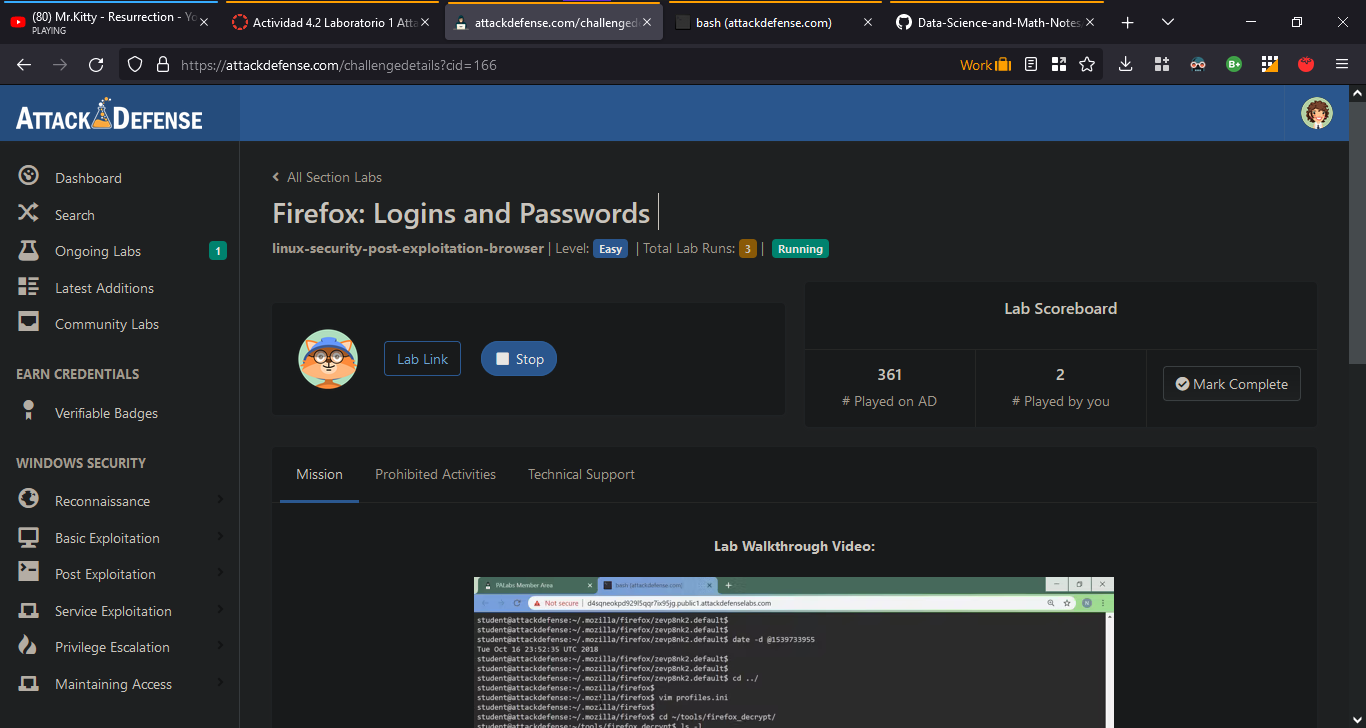
\includegraphics[scale=0.5]{img/firefox-evidence-before.png}
                \caption{Laboratorio antes de iniciar la actividad}
                \label{fig:firefox-before}
            \end{figure}
        \end{landscape}

        \begin{figure}[!h]
            \centering
            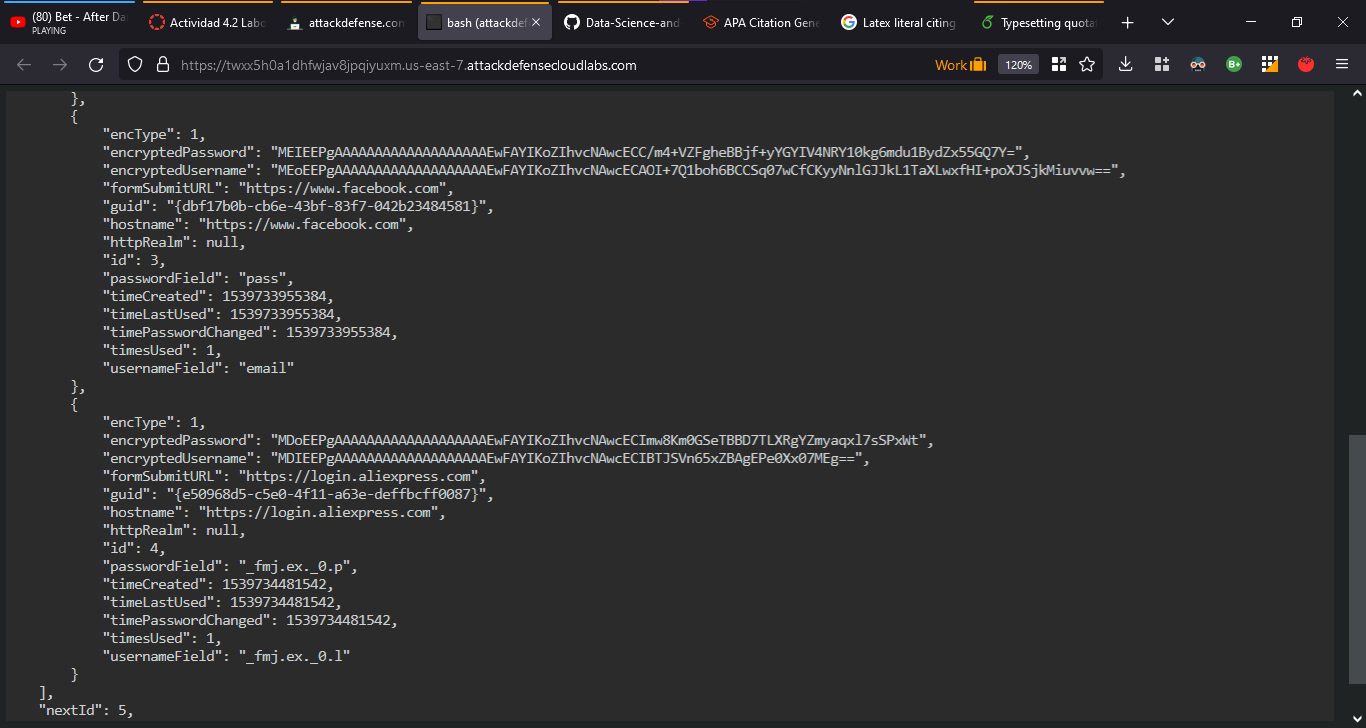
\includegraphics[scale=0.35]{img/aliexpress-username.png}
            \caption{Captura del nombre de usuario encriptado para el sitio \emph{aliexpress}}
            \label{fig:encrypted-ali}
        \end{figure}

        \begin{figure}[!h]
            \centering
            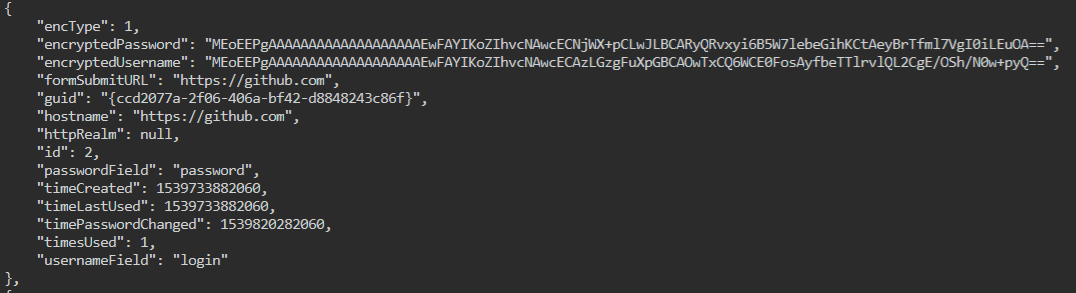
\includegraphics[scale=0.5]{img/github-password-changed.png}
            \caption{Contraseña alterada en el sitio \emph{GitHub}}
            \label{fig:github-password}
        \end{figure}

        \begin{figure}[!h]
            \centering
            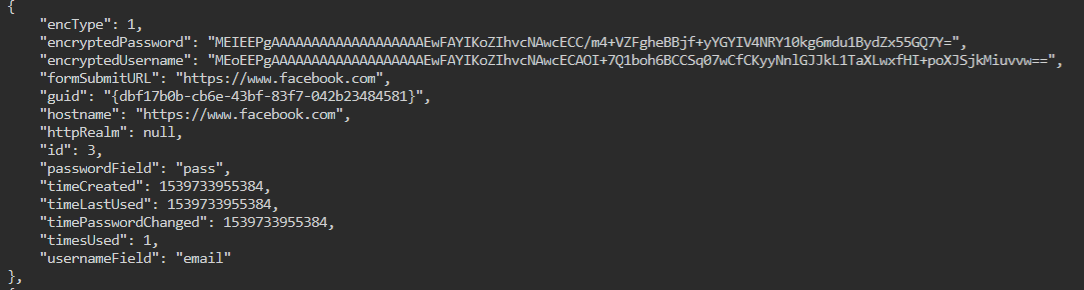
\includegraphics[scale=0.5]{img/facebook-last-used-unix.png}
            \caption{Última vez que se usó la contraseña para el sitio \emph{Facebook}}
            \label{fig:facebook-last-used}
        \end{figure}

        \clearpage
        \begin{figure}[!h]
            \centering
            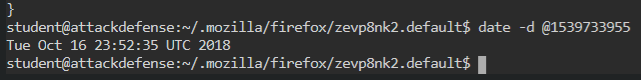
\includegraphics[scale=0.7]{img/facebook-last-used-converted.png}
            \caption{Fecha de último uso convertida al formato DD-MM-YY HH:MM:SS GMT}
            \label{fig:facebook-last-used-converted}
        \end{figure}

        \begin{figure}[!h]
            \centering
            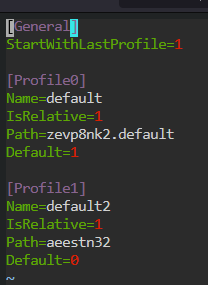
\includegraphics[scale=0.7]{img/profiles-before.png}
            \caption{Archivo \texttt{profiles.ini} original}
            \label{fig:profiles-before}
        \end{figure}

        \begin{figure}[!h]
            \centering
            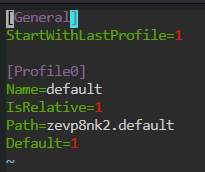
\includegraphics[scale=0.7]{img/profiles-after.png}
            \caption{Archivo \texttt{profiles.ini} después de borrar la última entrada}
            \label{fig:profiles-after}
        \end{figure}

        \clearpage
        \begin{figure}[!h]
            \centering
            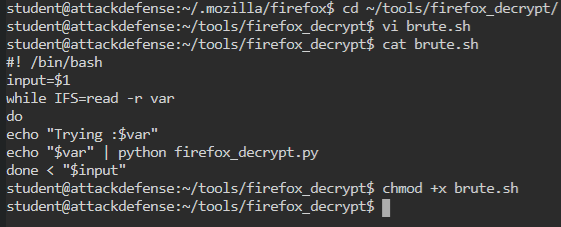
\includegraphics[scale=0.7]{img/bash-vim.png}
            \caption{Diseño de script de bash}
            \label{fig:bash-vim}
        \end{figure}

        \begin{figure}[!h]
            \centering
            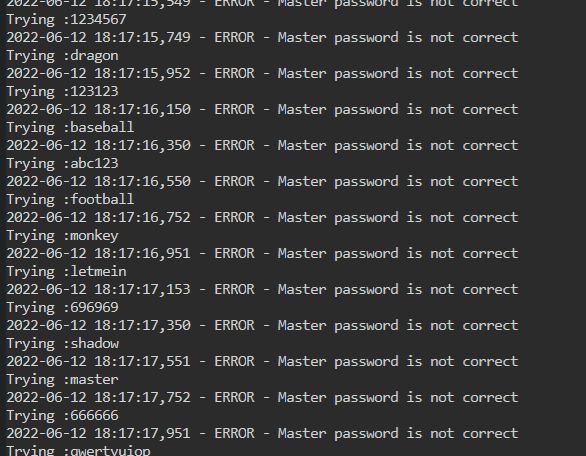
\includegraphics[scale=0.7]{img/brute-attempts.png}
            \caption{Intentos de fuerza bruta con diccionario}
            \label{fig:brute-attempts}
        \end{figure}
        
        \clearpage
        \begin{figure}[!h]
            \centering
            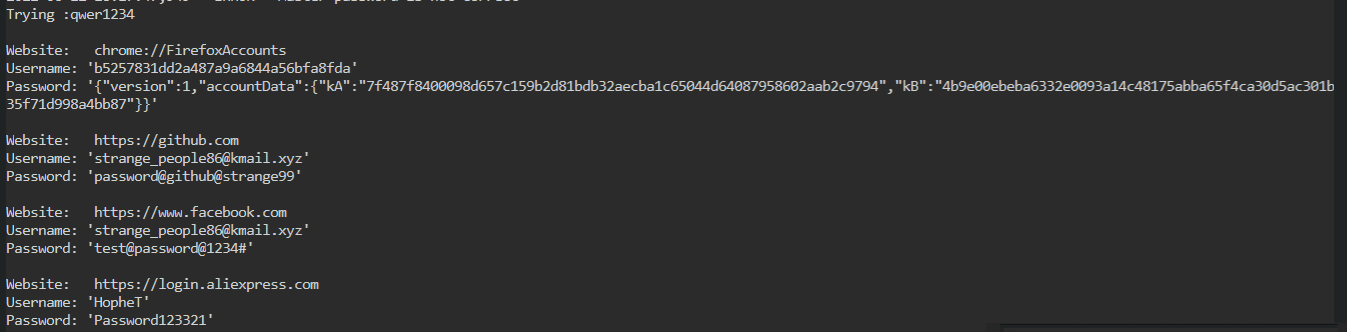
\includegraphics[scale=0.4]{img/brute-found.png}
            \caption{Clave encontrada}
            \label{fig:brute-found}
        \end{figure}

        \begin{landscape}
            \begin{figure}[!h]
                \centering
                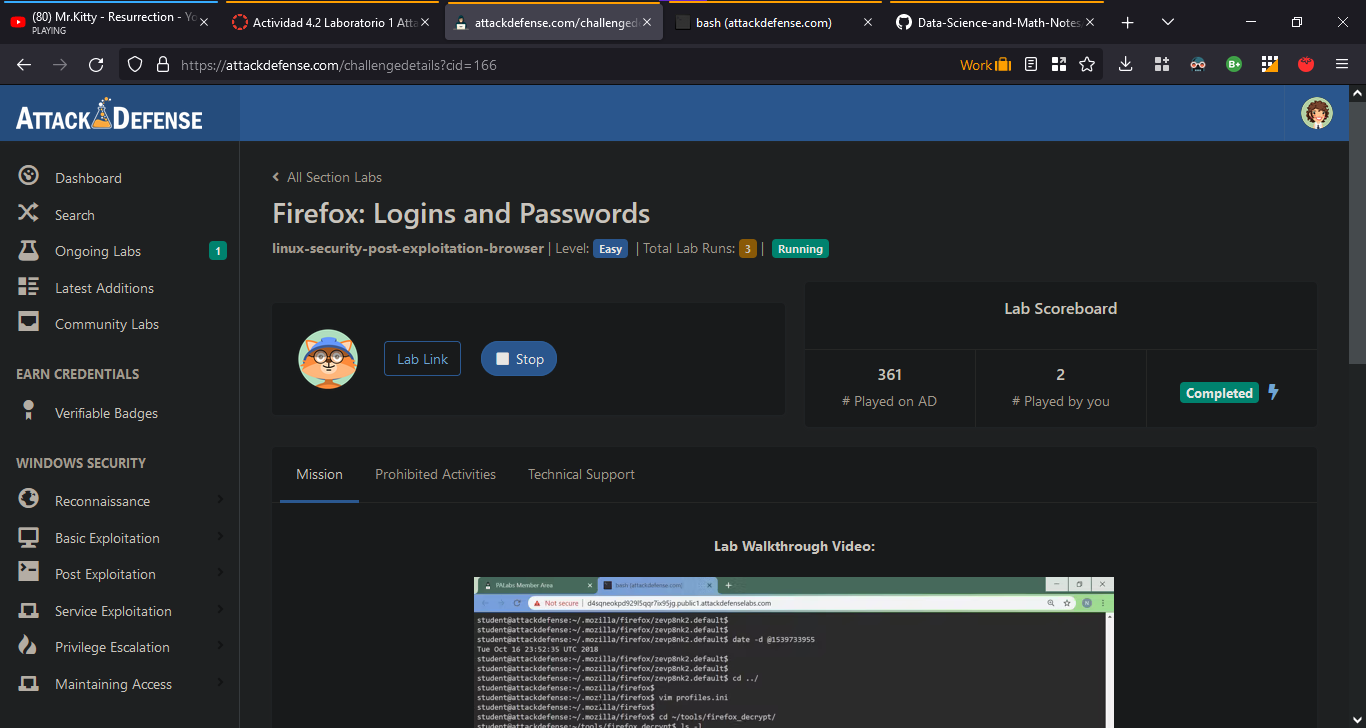
\includegraphics[scale=0.5]{img/firefox-evidence-after.png}
                \caption{Laboratorio después de completar la actividad}
                \label{fig:firefox-after}
            \end{figure}
        \end{landscape}

\end{document}
